\documentclass[../main.tex]{subfiles}
\begin{document}
\subsection{Polynomial regression}\label{subsec:pol_regression}
Check out this source \footnote{\url{https://en.wikipedia.org/wiki/Polynomial_regression}}.
The model function is chosen as a univariate polynomial of degree $m-1$ so that the goal of this type of regression is to find the optimal set of $m$ coefficients $\{c_{0},\dots,c_{m-1}\}$ that minimises the residual when $f(x,\mu=(c_{0},\dots,c_{m-1})) = \sum_{k=1}^{m}c_{k}x^{k-1}$.
When we fit such model to the $n$ pairs $\{(x_{j},y_{j})\}_{j=1,\dots,n}$ the problem can be written in matrix form as $\boldsymbol{Ac}-\boldsymbol{b}=\boldsymbol{r}\neq \boldsymbol{0}$ where
\begin{equation*}
        \mathbb{R}^{n\times m}\ni\underbrace{\boldsymbol{A} = \begin{bmatrix}
                        1 & x_{1} & x_{1}^{2} & \cdots & x_{1}^{m-2} & x_{1}^{m-1} \\
                        \vdots &\vdots & \vdots & \cdots & \vdots & \vdots \\
                        1 & x_{n} & x_{n}^{2} & \cdots & x_{n}^{m-2} & x_{n}^{m-1} \\
        \end{bmatrix}}_{\text{model matrix}}\,,\;\underbrace{\boldsymbol{c} = \begin{bmatrix}
                c_{0} \\
                \vdots \\
                c_{m-1}
        \end{bmatrix}}_{\text{parameters}}\,,\;\underbrace{\boldsymbol{b} = \begin{bmatrix}
                y_{1} \\
                \vdots \\
                y_{n}
\end{bmatrix}}_{\text{data}}\,.
\end{equation*}
Each column $k=1,\dots,m$ of the model matrix $\boldsymbol{A}$ might be thought as the values that a given basis function $\phi_{k}(x)$ takes in correspondance of the data i.e. $A_{jk} = \phi_{k}(x_{j})$.
The model function can thus be written in such basis as $f(x, (c_{0},\dots,c_{m-1})) = \sum_{k=1}^{m-1}c_{k}\phi_{k}(x)$.
The system is overdetermined due to the fact that $\boldsymbol{A}$ is tall and skinny ($n\gg m$) and therefore a solution $\boldsymbol{c}$ is guaranteed to exist if and only if $\boldsymbol{A}$ is full rank.
\begin{figure}[H]
    \centering 
    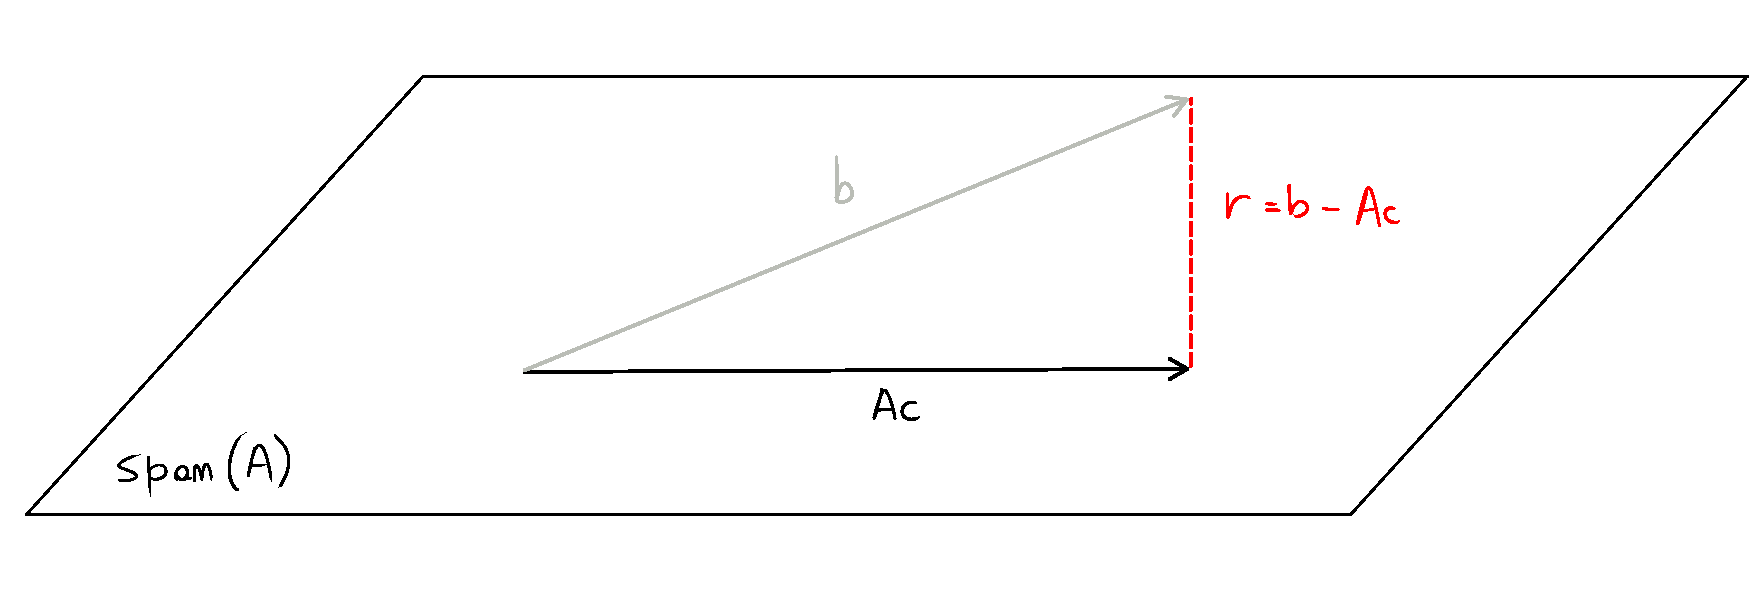
\includegraphics[keepaspectratio, width=\textwidth]{../figures/fig2.5.2.1.pdf}
    \caption{Visual relationship between the data $\boldsymbol{b}\in \mathbb{R}^{n}$, the least-squares solution $\boldsymbol{c}\in \mathbb{R}^{m}$ and its residual $\boldsymbol{r}\in \mathbb{R}^{n}$. The transformation $\boldsymbol{Ac}$ lives in $\text{span}(\boldsymbol{A})$ but $\boldsymbol{b}$ does not because $n\gg m$. To find the closest $\boldsymbol{x}\in \text{span}(\boldsymbol{A})$ to $\boldsymbol{b}$ we look for the orthogonal projection of $\boldsymbol{b}$ on $\text{span}(\boldsymbol{A})$ and by minimising the norm of such distance give by $\boldsymbol{r}=\boldsymbol{b}-\boldsymbol{Ax}$.}
    \label{fig2.5.2.1}
\end{figure}
Such solution is not unique and we are interested in finding the one that minimises the residual vector $\boldsymbol{r}$ in the $L_{2}-$norm sense.
To do that we derive the analytical expression of such norm 
\begin{align}
     ||\boldsymbol{r}||^{2} =&\, \boldsymbol{r}^{T}\boldsymbol{r} = \big(\boldsymbol{b}-\boldsymbol{Ac}\big)^{T}\big(\boldsymbol{b}-\boldsymbol{Ac}\big) = \big(\boldsymbol{b}^{T} -\boldsymbol{c}^{T}\boldsymbol{A}^{T}\big)\big(\boldsymbol{b}-\boldsymbol{Ac}\big)\nonumber \\
                            =&\, \boldsymbol{b}^{T}\boldsymbol{b} - \boldsymbol{b}^{T}\boldsymbol{Ac} - \boldsymbol{c}^{T}\boldsymbol{A}^{T}\boldsymbol{b} + \boldsymbol{c}^{T}\boldsymbol{A}^{T}\boldsymbol{A}\boldsymbol{c} \,, \label{eq2.5.2.1} 
\end{align}
We notice that since $\boldsymbol{c}^{T}\boldsymbol{A}^{T}\boldsymbol{b} = (\boldsymbol{A}\boldsymbol{c})^{T}\boldsymbol{b}$ is a number it will be equal to its transpose $\boldsymbol{b}^{T}\boldsymbol{Ac}$ which reduces \eqref{eq2.5.2.1} to 
\begin{equation}\label{eq2.5.2.2}
        ||\boldsymbol{r}||^{2} = \boldsymbol{b}^{T}\boldsymbol{b} - 2\boldsymbol{b}^{T}\boldsymbol{Ac} + \boldsymbol{c}^{T}\underbrace{\boldsymbol{A}^{T}\boldsymbol{A}}_{\text{sym.}}\boldsymbol{c} = \boldsymbol{b}^{T}\boldsymbol{b} - 2\boldsymbol{b}^{T}\boldsymbol{Ac} + \boldsymbol{c}^{T}\big(\boldsymbol{A}^{T}\boldsymbol{A}\big)^T\boldsymbol{c} =: r(\boldsymbol{c})\,,
\end{equation}
where in the last equality we emphasize that the (squared) norm of the residual is a scalar quadratic function of the parameter vector $\boldsymbol{c}$.
The quadratic dependence on $\boldsymbol{c}$ is encoded by the presence of the bilinear form \footnote{\url{https://en.wikipedia.org/wiki/Bilinear_form}}
\begin{align*}
        a : V\times V &\to \mathbb{R} \nonumber \\
            \boldsymbol{x},\boldsymbol{y} &\mapsto \boldsymbol{x}^{T}\big(\boldsymbol{A}^{T}\boldsymbol{A}\big)^{T}\boldsymbol{y} \,,
\end{align*}
and its associated quadratic form \footnote{\url{https://en.wikipedia.org/wiki/Quadratic_form}}
\begin{align*}
        q : V &\to \mathbb{R} \nonumber \\
        \boldsymbol{x} &\mapsto a(\boldsymbol{x},\boldsymbol{x}) = \boldsymbol{x}^{T}\big(\boldsymbol{A}^{T}\boldsymbol{A}\big)^{T}\boldsymbol{x}\,.
\end{align*}
The minimum of \eqref{eq2.5.2.2} is found by computing its gradient
\begin{equation*}
     \nabla r(\boldsymbol{c}) = 2 \boldsymbol{c}^{T}\boldsymbol{A}^{T}\boldsymbol{A} - 2 \boldsymbol{b}^{T}\boldsymbol{A}\,,
\end{equation*}
and imposing the equality to $0$ yieling the so-called \textbf{normal equations}
\begin{equation}\label{eq2.5.2.3}
        \boldsymbol{c} = \argmin_{\boldsymbol{x}\in \mathbb{R}^{m}}r(\boldsymbol{x}) = \big(\boldsymbol{A}^{T}\boldsymbol{A}\big)^{-1}\boldsymbol{A}^{T}\boldsymbol{b} = \boldsymbol{A}^{+}\boldsymbol{b} \,,
\end{equation}
where $\big(\boldsymbol{A}^{T}\boldsymbol{A}\big)^{-1}\boldsymbol{A}^{T} =: \boldsymbol{A}^{+}\in \mathbb{R}^{m\times n}$ is the pseudoinverse of a non-square matrix $\boldsymbol{A}\in \mathbb{R}^{n\times m}$ of rank $m$.

% Statistical error analysis 
\subfile{subsubsec:stat_err_analysis}
\end{document}
